% ============================================================================
%  sections/chapitre2.tex
% ============================================================================
\chapter{Architecture et Base de données}
\label{chapitre-2-architecture-et-base-de-donnees}

\section{Introduction}
\label{introduction-ch2}

Ce chapitre détaille l'architecture technique de la plateforme, le choix des technologies, l'organisation modulaire du code et le dictionnaire complet des modèles Django.

\begin{figure}[htbp]
  \centering
  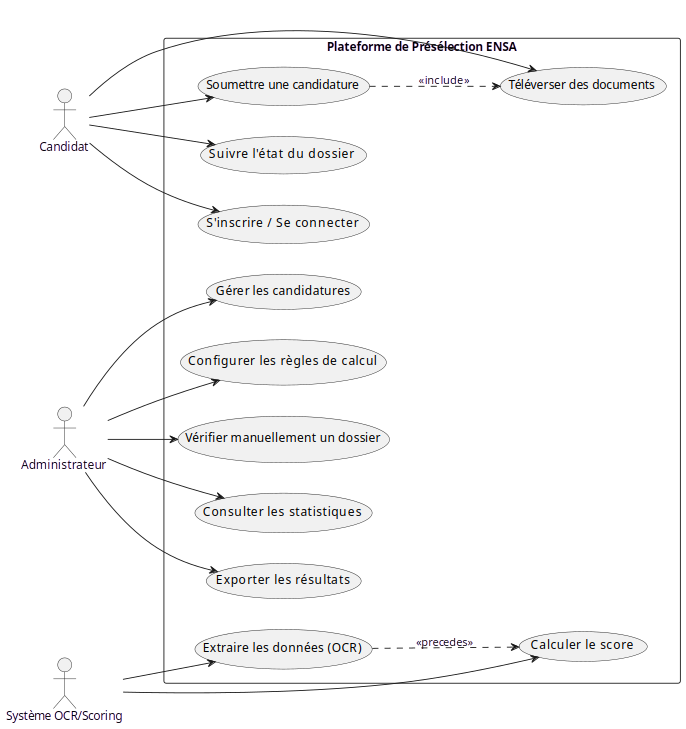
\includegraphics[width=0.8\textwidth]{media/image3.png}
  \caption{Diagramme de cas d'utilisation global de la plateforme}
  \label{fig:use-cases}
\end{figure}

\section{Architecture globale}
\label{architecture-globale}

\subsection{Vue d'ensemble}
\label{vue-densemble}

L'application repose sur une architecture moderne Full-Stack Client-Serveur à trois niveaux :

\begin{itemize}
  \item Frontend : React 18 compilé via Vite, avec Tailwind CSS pour le rendu responsive. L'architecture s'appuie sur des composants réutilisables, React Router v6 et un state management optimisé via Context API.
  \item Backend : Django 4.2 LTS et Django REST Framework (DRF), exposant une API REST sécurisée par JWT (SimpleJWT). Le backend est organisé en 5 applications Django indépendantes.
  \item Base de données : PostgreSQL 15 géré par l'ORM Django, assurant la persistance des candidatures, configurations et historiques.
  \item Temps réel : Django Channels 4.0 avec Redis comme channel layer pour les WebSockets (notifications en temps réel avec barre de progression).
\end{itemize}

\begin{figure}[htbp]
  \centering
  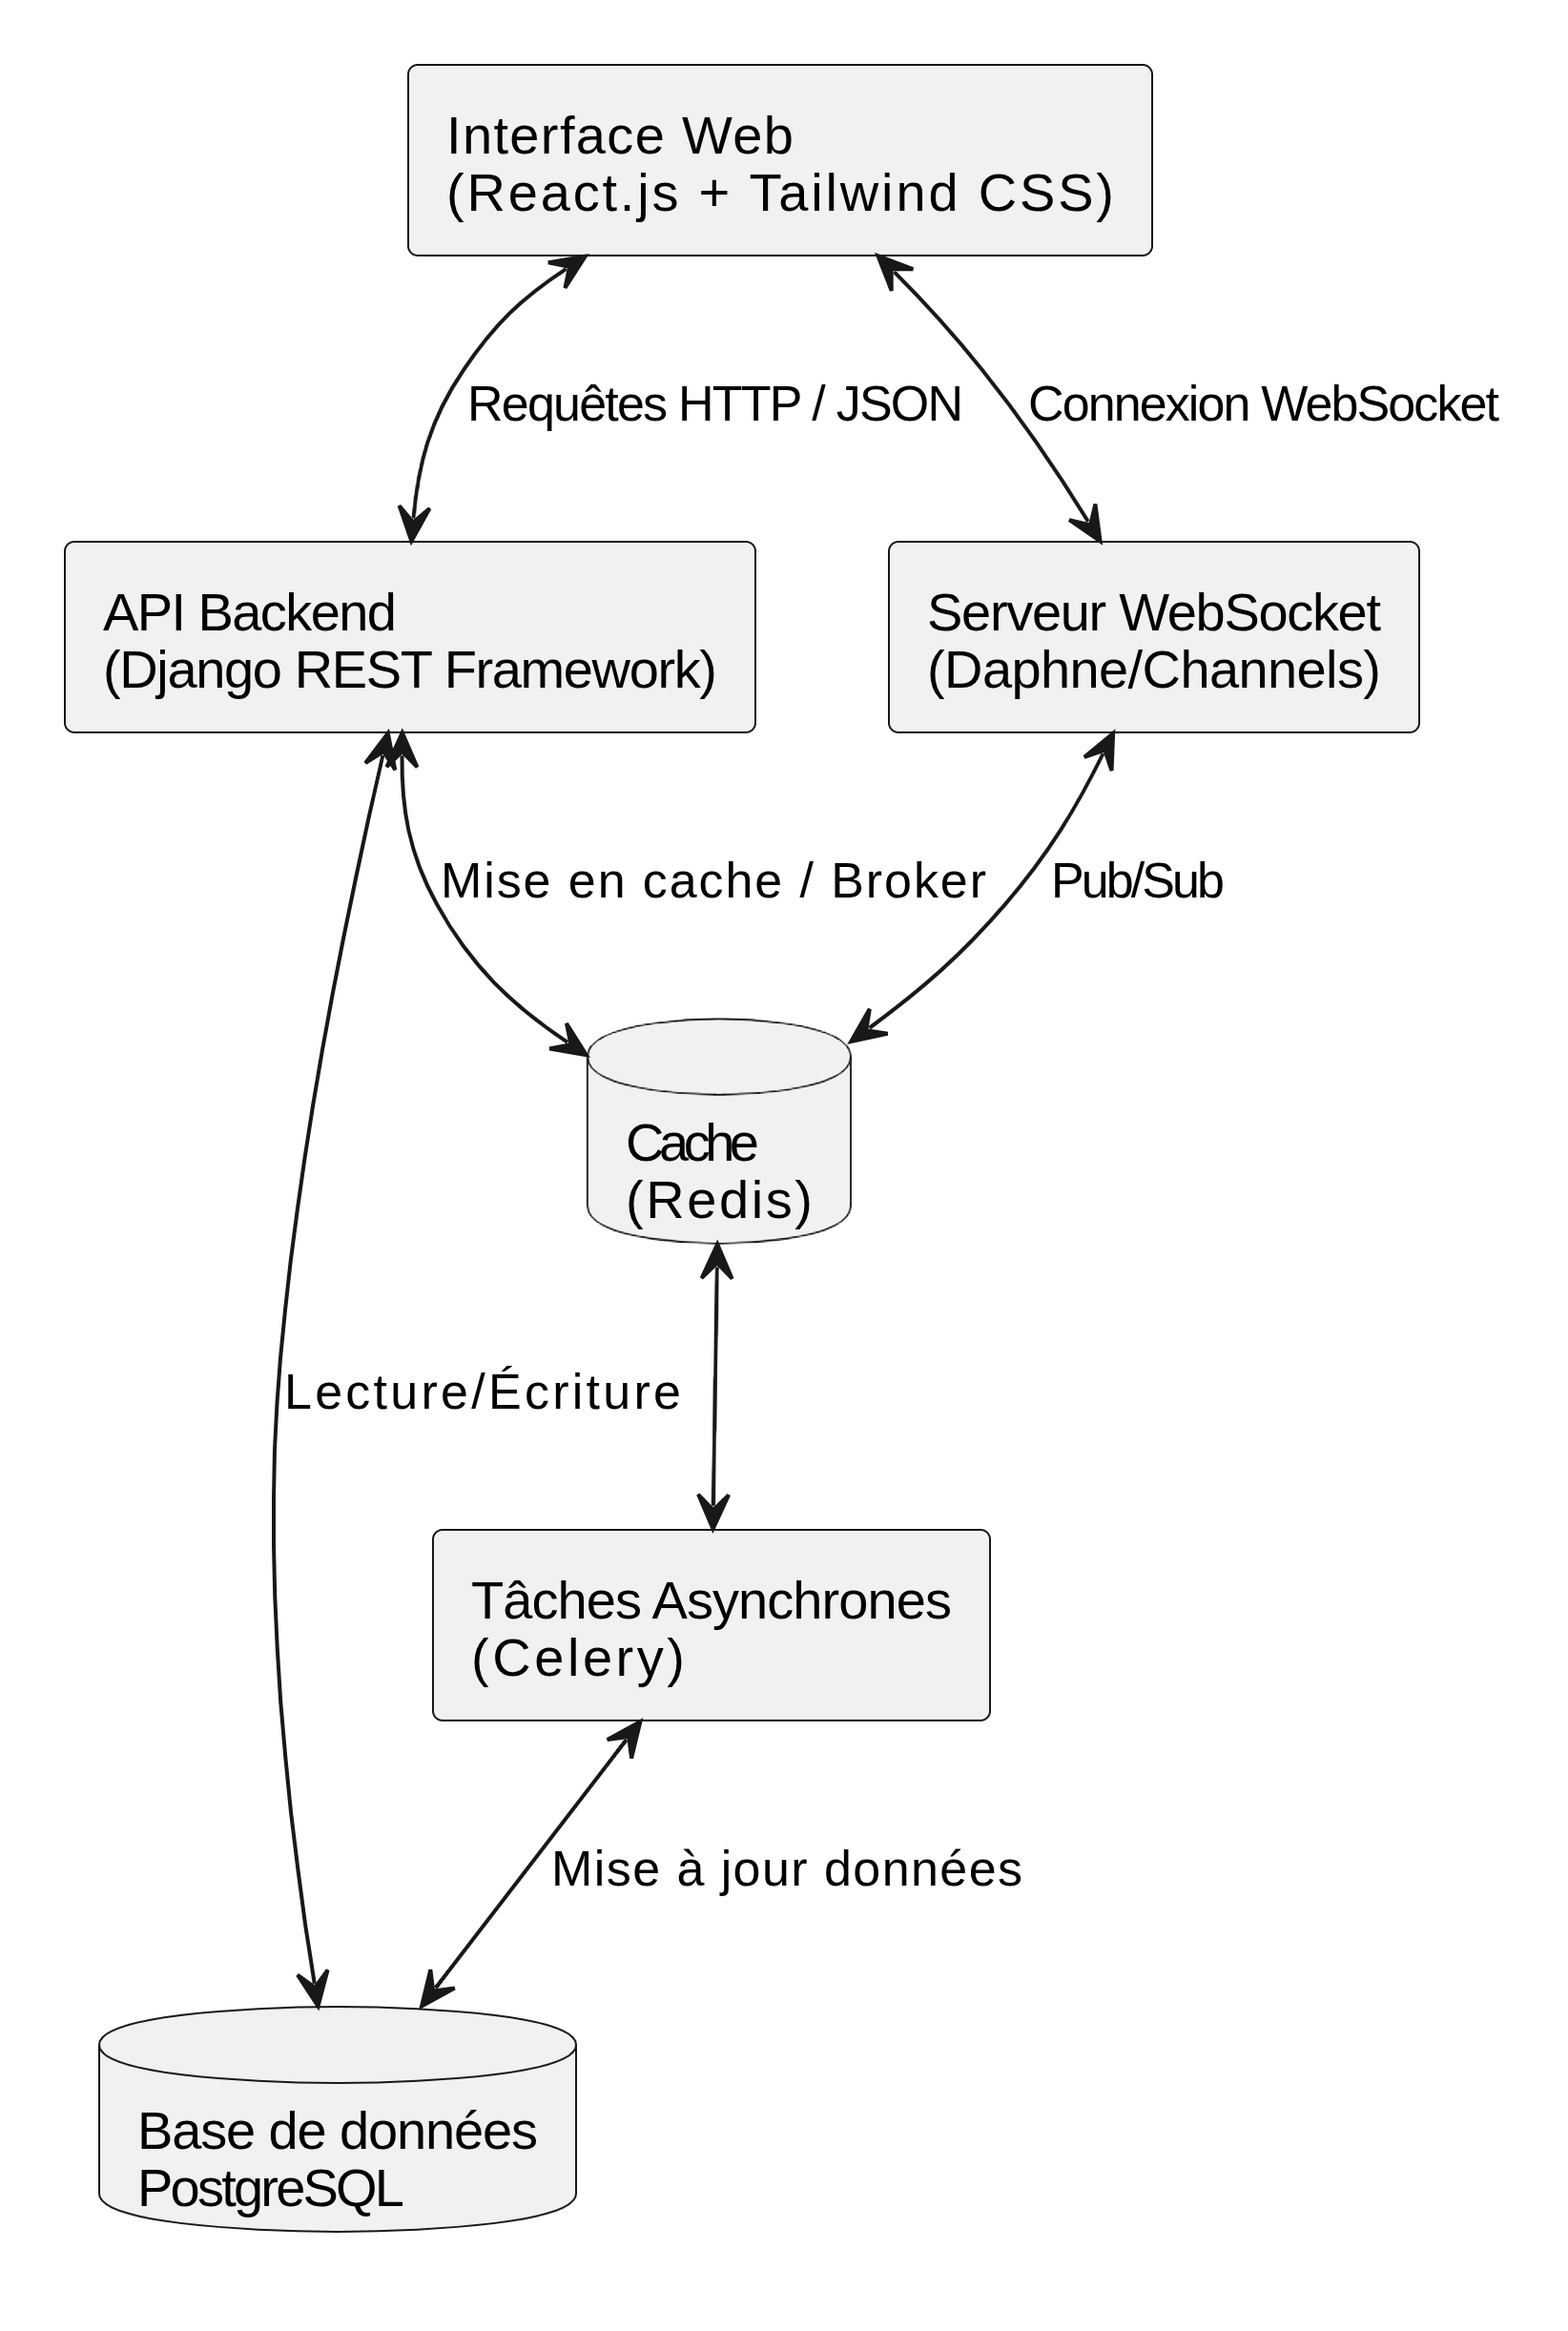
\includegraphics[width=0.6\textwidth]{media/image5.png}
  \caption{Architecture générale de la plateforme de présélection}
  \label{fig:architecture}
\end{figure}

\subsection{Architecture REST stateless}
\label{architecture-rest-stateless}

Le frontend communique avec le backend exclusivement via des endpoints REST sécurisés par JWT. Les réponses sont au format JSON. Le pattern est strictement stateless côté serveur, à l'exception des connexions WebSocket persistantes pour les notifications.

\section{Stack technologique}
\label{stack-technologique}

\begin{table}[htbp]
  \centering
  \caption{Stack technologique du projet}
  \begin{tabularx}{\textwidth}{@{} l l X @{}}
    \toprule
    \textbf{Technologie} & \textbf{Version} & \textbf{Rôle} \\
    \midrule
    Django & 4.2 LTS & Framework backend principal \\
    Django REST Framework & 3.17 & Construction de l'API REST \\
    Django Channels & 4.0 & WebSockets temps réel \\
    SimpleJWT & 5.5 & Authentification par tokens JWT \\
    React & 18 & Framework frontend SPA \\
    Tailwind CSS & 3.x & Framework CSS utilitaire \\
    PostgreSQL & 15 & Base de données relationnelle \\
    Redis & 7.x & Channel Layer WebSocket \\
    pdfplumber + pytesseract & --- & Extraction OCR \\
    fuzzywuzzy & 0.18 & Correspondance floue des matières \\
    openpyxl & --- & Import/Export Excel \\
    \bottomrule
  \end{tabularx}
  \label{tab:stack}
\end{table}

\section{Organisation modulaire du backend}
\label{organisation-modulaire-du-backend}

Le backend est structuré en 5 applications Django indépendantes, chacune gérant un domaine métier spécifique :

\begin{table}[htbp]
  \centering
  \caption{Applications Django du backend}
  \begin{tabularx}{\textwidth}{@{} l X l @{}}
    \toprule
    \textbf{Application} & \textbf{Responsabilité} & \textbf{Fichiers clés} \\
    \midrule
    users & Authentification, comptes, profils candidats & models.py, serializers.py, views.py \\
    candidatures & Dossiers, documents, notes, services métier & models.py, views.py, services/ \\
    administration & Filières, diplômes, épreuves, historique & models.py, views.py \\
    scoring & Règles de rejet, configuration scoring & models.py, views.py \\
    notifications & Notifications email et WebSocket & models.py, consumers.py, views.py \\
    \bottomrule
  \end{tabularx}
  \label{tab:apps-django}
\end{table}

Le répertoire \texttt{candidatures/services/} contient la logique métier critique :

\begin{table}[htbp]
  \centering
  \caption{Services métier du module candidatures}
  \begin{tabularx}{\textwidth}{@{} l l X @{}}
    \toprule
    \textbf{Service} & \textbf{Fichier} & \textbf{Rôle} \\
    \midrule
    Extraction OCR & extraction.py & Extraction des informations depuis les documents scannés \\
    Fuzzy Matching & fuzzy\_matching.py & Correspondance floue des noms de matières \\
    Règles de rejet & regles.py & Application des 7 types de règles de rejet automatique \\
    Scoring & scoring.py & Calcul du score pondéré par filière \\
    Vérification & verification\_document.py & Vérification d'authenticité des documents \\
    Invitation PDF & invitation\_pdf.py & Génération des convocations au format PDF \\
    \bottomrule
  \end{tabularx}
  \label{tab:services}
\end{table}

\begin{figure}[htbp]
  \centering
  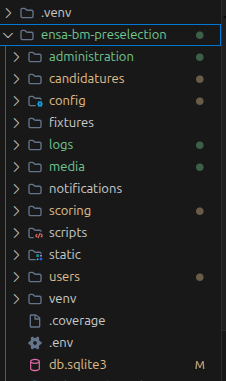
\includegraphics[width=0.6\textwidth]{media/image6.png}
  \caption{Organisation modulaire du backend Django}
  \label{fig:modules-django}
\end{figure}

\section{Dictionnaire des modèles Django}
\label{dictionnaire-des-modeles-django}

Le modèle relationnel est structuré autour de 12 entités principales réparties dans les applications Django. Nous détaillons ci-dessous chaque modèle.

\subsection{Application Users}
\label{application-users}

Le modèle \texttt{User} étend \texttt{AbstractBaseUser} de Django pour personnaliser l'authentification. L'identification se fait par email et CIN (Carte d'Identité Nationale). Trois rôles sont définis : CANDIDAT, RESPONSABLE et ADMIN, implémentant un contrôle d'accès RBAC.

\begin{table}[htbp]
  \centering
  \caption{Modèle User}
  \begin{tabularx}{\textwidth}{@{} l l X @{}}
    \toprule
    \textbf{Attribut} & \textbf{Type} & \textbf{Contrainte} \\
    \midrule
    id & UUID & Clé primaire auto-générée \\
    email & VARCHAR & UNIQUE, NOT NULL \\
    cin & VARCHAR & UNIQUE, NOT NULL \\
    role & ENUM & CANDIDAT / RESPONSABLE / ADMIN \\
    is\_active & BOOLEAN & Défaut : True \\
    password & VARCHAR & Hashé via PBKDF2 \\
    \bottomrule
  \end{tabularx}
  \label{tab:model-user}
\end{table}

Le modèle \texttt{Candidat} est relié en OneToOne à \texttt{User} et stocke le profil détaillé :

\begin{table}[htbp]
  \centering
  \caption{Modèle Candidat}
  \begin{tabularx}{\textwidth}{@{} l l X @{}}
    \toprule
    \textbf{Attribut} & \textbf{Type} & \textbf{Contrainte} \\
    \midrule
    id & UUID & Clé primaire \\
    user\_id & FK $\rightarrow$ User & OneToOne, CASCADE \\
    nom & VARCHAR & NOT NULL \\
    prenom & VARCHAR & NOT NULL \\
    telephone & VARCHAR & Optionnel \\
    date\_naissance & DATE & NOT NULL \\
    \bottomrule
  \end{tabularx}
  \label{tab:model-candidat}
\end{table}

\subsection{Application Candidatures}
\label{application-candidatures}

Le modèle \texttt{Dossier} est le modèle central de l'application. Il lie un \texttt{Candidat} à une \texttt{Filiere} et contient le statut, les scores calculés et les motifs de rejet éventuels.

\begin{table}[htbp]
  \centering
  \caption{Modèle Dossier}
  \begin{tabularx}{\textwidth}{@{} l l X @{}}
    \toprule
    \textbf{Attribut} & \textbf{Type} & \textbf{Contrainte} \\
    \midrule
    id & UUID & Clé primaire \\
    candidat\_id & FK $\rightarrow$ Candidat & CASCADE \\
    filiere\_id & FK $\rightarrow$ Filiere & CASCADE \\
    statut & ENUM & 11 valeurs possibles \\
    score & DECIMAL & Score dossier calculé \\
    score\_final & DECIMAL & 40\% dossier + 60\% épreuve \\
    rang\_final & INT & Classement par filière \\
    mention & ENUM & Auto-calculé \\
    moyenne\_generale & DECIMAL & Moyenne des semestres \\
    \bottomrule
  \end{tabularx}
  \label{tab:model-dossier}
\end{table}

Le modèle \texttt{Document} gère les pièces justificatives uploadées par le candidat :

\begin{table}[htbp]
  \centering
  \caption{Modèle Document}
  \begin{tabularx}{\textwidth}{@{} l l X @{}}
    \toprule
    \textbf{Attribut} & \textbf{Type} & \textbf{Contrainte} \\
    \midrule
    id & UUID & Clé primaire \\
    dossier\_id & FK $\rightarrow$ Dossier & CASCADE \\
    type\_doc & ENUM & DIPLOME / RELEVE / CIN / PHOTO \\
    fichier & FILE & Stocké dans media/dossiers/\{uuid\}/ \\
    qualite\_ocr & DECIMAL & Score de confiance OCR \\
    \bottomrule
  \end{tabularx}
  \label{tab:model-document}
\end{table}

\begin{figure}[htbp]
  \centering
  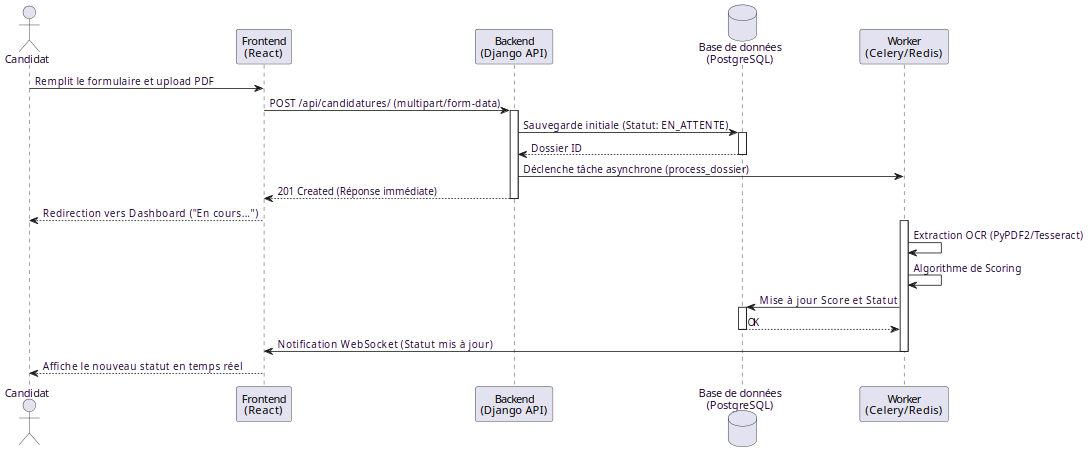
\includegraphics[width=0.9\textwidth]{media/image7.png}
  \caption{Diagramme de classes de la plateforme}
  \label{fig:class-diagram}
\end{figure}

Le modèle \texttt{NoteSemestre} remplace l'ancienne approche par \texttt{NoteMatiere}. Il intègre la moyenne par semestre, la session et la mention calculée dynamiquement :

\begin{table}[htbp]
  \centering
  \caption{Modèle NoteSemestre}
  \begin{tabularx}{\textwidth}{@{} l l X @{}}
    \toprule
    \textbf{Attribut} & \textbf{Type} & \textbf{Contrainte} \\
    \midrule
    id & UUID & Clé primaire \\
    dossier\_id & FK $\rightarrow$ Dossier & CASCADE \\
    semestre & ENUM & S1 à S6 \\
    moyenne & DECIMAL & Plage stricte [10.00, 20.00] \\
    session & ENUM & NORMALE / RATTRAPAGE \\
    mention & ENUM & Auto-calculé (editable=False) \\
    \bottomrule
  \end{tabularx}
  \label{tab:model-notesemestre}
\end{table}

\subsection{Application Administration et Scoring}
\label{application-administration-et-scoring}

Le modèle \texttt{Filiere} définit les filières du cycle ingénieur avec leurs paramètres :

\begin{table}[htbp]
  \centering
  \caption{Modèle Filiere}
  \begin{tabularx}{\textwidth}{@{} l l X @{}}
    \toprule
    \textbf{Attribut} & \textbf{Type} & \textbf{Contrainte} \\
    \midrule
    id & UUID & Clé primaire \\
    nom & VARCHAR & NOT NULL \\
    code & VARCHAR & UNIQUE (TDI, IACS, IAA, G2ER) \\
    niveau & ENUM & BAC2 / BAC3 \\
    places\_disponibles & INT & Défaut : 30 \\
    \bottomrule
  \end{tabularx}
  \label{tab:model-filiere}
\end{table}

Les modèles \texttt{EpreuveEcrite} et \texttt{NoteEcrite} gèrent la logistique du concours écrit :

\begin{table}[htbp]
  \centering
  \caption{Modèles d'administration et scoring}
  \begin{tabularx}{\textwidth}{@{} l l X @{}}
    \toprule
    \textbf{Modèle} & \textbf{Attributs clés} & \textbf{Rôle} \\
    \midrule
    EpreuveEcrite & nom, date\_epreuve, seuil\_admission, statut & Gestion de l'épreuve par filière \\
    NoteEcrite & note, resultat, rang\_final & Note individuelle et classement \\
    ConfigScoring & matiere, poids, bonus\_mention & Pondération scoring par filière \\
    RegleRejet & type\_regle, parametre, is\_active, message & Règle de rejet configurable \\
    HistoriqueAction & action, commentaire, timestamp & Traçabilité des décisions \\
    \bottomrule
  \end{tabularx}
  \label{tab:model-admin}
\end{table}

\section{Relations et cardinalités}
\label{relations-et-cardinalites}

\begin{table}[htbp]
  \centering
  \caption{Relations et cardinalités du modèle de données}
  \begin{tabularx}{\textwidth}{@{} l l X @{}}
    \toprule
    \textbf{Relation} & \textbf{Type} & \textbf{Cardinalité} \\
    \midrule
    User $\rightarrow$ Candidat & OneToOne & 1..1 \\
    Candidat $\rightarrow$ Dossier & OneToMany & 1..* \\
    Dossier $\rightarrow$ Document & OneToMany & 1..4 \\
    Dossier $\rightarrow$ NoteSemestre & OneToMany & 1..6 \\
    Filiere $\rightarrow$ Dossier & OneToMany & 1..* \\
    Filiere $\rightarrow$ RegleRejet & OneToMany & 1..* \\
    Filiere $\rightarrow$ EpreuveEcrite & OneToMany & 1..* \\
    EpreuveEcrite $\rightarrow$ NoteEcrite & OneToMany & 1..* \\
    Dossier $\rightarrow$ HistoriqueAction & OneToMany & 1..* \\
    User $\rightarrow$ Notification & OneToMany & 1..* \\
    \bottomrule
  \end{tabularx}
  \label{tab:relations}
\end{table}

\section{Machine d'états du dossier}
\label{machine-detats-du-dossier}

Le dossier suit une machine d'états stricte implémentée dans la méthode \texttt{changer\_statut()} du modèle. Chaque transition crée automatiquement un enregistrement \texttt{HistoriqueAction} pour la traçabilité :

\begin{table}[htbp]
  \centering
  \caption{Machine d'états du dossier de candidature}
  \begin{tabularx}{\textwidth}{@{} l X @{}}
    \toprule
    \textbf{État} & \textbf{Transitions possibles} \\
    \midrule
    BROUILLON & $\rightarrow$ EN\_TRAITEMENT (soumission) \\
    EN\_TRAITEMENT & $\rightarrow$ REJETE\_AUTO | EN\_ATTENTE | INCOMPLET | SUSPECT \\
    INCOMPLET & $\rightarrow$ EN\_TRAITEMENT (complétion) \\
    SUSPECT & $\rightarrow$ EN\_ATTENTE | REJETE\_FINAL (décision manuelle) \\
    EN\_ATTENTE & $\rightarrow$ PRESELECTIONNE | REJETE\_FINAL \\
    PRESELECTIONNE & $\rightarrow$ ADMIS\_FINAL | RECALE\_FINAL | ABSENT\_ECRIT \\
    \bottomrule
  \end{tabularx}
  \label{tab:machine-etats}
\end{table}

\begin{figure}[htbp]
  \centering
  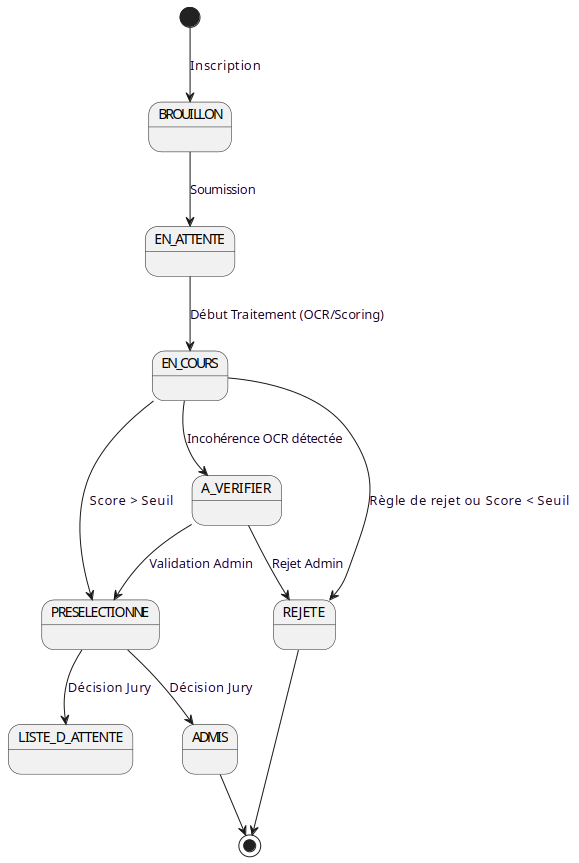
\includegraphics[width=0.6\textwidth]{media/image9.png}
  \caption{Machine d'états du dossier de candidature}
  \label{fig:state-machine}
\end{figure}

\section{Conclusion}
\label{conclusion-ch2}

Ce chapitre a détaillé l'architecture Full-Stack de la plateforme et le modèle de données relationnel complet. L'organisation modulaire en 5 applications Django assure une séparation claire des responsabilités. Le chapitre suivant présentera la logique métier et les algorithmes de scoring et d'OCR.
